\documentclass[border=4pt]{standalone}
\usepackage[T1]{fontenc}
\usepackage{helvet}
\renewcommand{\familydefault}{\sfdefault}
\usepackage{graphicx}
\usepackage{caption}
\usepackage{amsmath}
\captionsetup{font={sf,footnotesize},labelfont={sf,bf,footnotesize},justification=justified,singlelinecheck=false}
\begin{document}
\setcounter{figure}{1}
\renewcommand{\thefigure}{S\arabic{figure}}
\begin{minipage}{7.20in}
\centering
\begin{figure}[htbp]
    \centering
    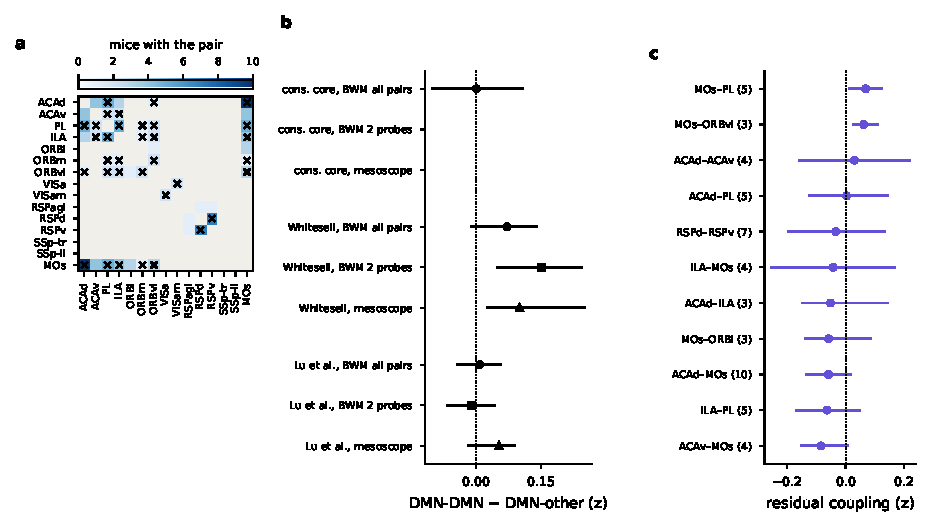
\includegraphics[width=\linewidth]{figS2_whitesell_coupling_panels.pdf}
    \caption{\textbf{a} Grey-screen region pairs within the Whitesell et al. DMN: mice with the pair (grey: never recorded); orange crosses, recorded on two probes in at least one session. 24 of 105 edges are recorded, 11 in $\geq$3 mice; those are all frontal-frontal (ACA, PL, ILA, ORB, MOs) or RSPd-RSPv, and no frontal-posterior edge is recorded at all. \textbf{b} DMN-DMN minus DMN-other coupling for three definitions: BWM cortical pairs (circles), BWM pairs on two probes (squares) and mesoscope (triangles; 13 sessions, 7 mice): 95\% mouse-bootstrap CI. For Whitesell, the two-probe excess (+0.15) comes 72\% from two frontal multi-probe sessions (KS046, SWC\_038; 6 mice in all), and the mesoscope excess mainly from one mouse (SP054, SSp-tr/VISa/VISam pairs). \textbf{c} Every Whitesell DMN edge recorded in $\geq$3 mice (number of mice in brackets): mean residual coupling over mice and 95\% bootstrap CI.}
    \label{fig:grey_s2}
\end{figure}
\end{minipage}
\end{document}
